\documentclass[10pt]{iopart}
\usepackage{graphicx}
\usepackage{booktabs}
\usepackage{dblfloatfix}
%\newcommand{\gguide}{{\it Preparing graphics for IOP Publishing journals}}
%Uncomment next line if AMS fonts required
\usepackage{iopams}
\begin{document}


\title[B A Urazbekov \etal ]{
Clusterization and Strong Coupled-Channels Effects in Deuteron Interaction with $^9$Be Nuclei
%Investigation of the Cluster Structure of $^9$Be by Reactions with a Deuteron Beam
}

\author{B~A~Urazbekov$^{1,2,3}$, A~S~Denikin$^{2,3}$, S~M~Lukyanov$^3$,  N~Itaco$^1$,  D~M~Janseitov$^{3,4}$, K~Mendibayev$^{3,5,6}$, V~Burjan$^7$, V~Kroha$^7$, J~Mrazek$^7$, W~H~Trzaska$^8$, M~N~Harakeh$^9$, D~Etasse$^{10}$, I~Stefan$^{11}$, D~Verney$^{11}$, T~ Issatayev$^{3,5}$, Yu~E~Penionzhkevich$^{3}$, K~A~Kuterbekov$^{5}$ and T~Zholdybayev$^{6}$}

\address{$^1$ Dipartimento di Matematica e Fisica,
Universit\`{a} degli Studi della Campania “Luigi Vanvitelli”, I-8110 Caserta, Italy}
\address{$^2$ Dubna State University, 141982 Dubna, Russia}
\address{$^3$ Joint Institute for nuclear research, 141980 Dubna, Russia}
\address{$^4$ Al-Farabi Kazakh National University, 050040 Almaty, Kazakhstan}
\address{$^5$ L~N~Gumilyov Eurasian National University, 010008 Nur-Sultan, Kazakhstan}
\address{$^6$ Institute of Nuclear Physics, 050032 Almaty, Kazakhstan}
\address{$^7$ Nuclear Physics Institute CAS, 25068 \v{R}e\v{z}, Czech Republic}
\address{$^8$ Department of Physics, University of Jyv\"askyl\"a, FIN-40014 Jyv\"askyl\"a, Finland}
\address{$^9$ KVI-CART, University of Groningen, 9747 AA Groningen, The Netherlands}
\address{$^{10}$ Normandie Universit\'{e}, ENSICAEN, UNICAEN, CNRS/IN2P3, LPC Caen, 14000 Caen, France}
\address{$^{11}$ Institut de Physique Nucl\'{e}aire, Univ. Paris-Sud, Universit\'{e} Paris-Saclay, F-91406 Orsay, France}
\ead{bakytzhan.urazbekov@gmail.com}

\begin{abstract}
Angular distributions of protons, deuterons, tritons and alpha particles emitted in the $d$ + $^{9}$Be reaction  at E$_{lab}$=19.5 and 35.0 MeV have been measured.
 The elastic scattering channel is analysed in the framework of both the Optical Model and  the Coupled-Channel approach. 
 The interaction potential of the $d$ + $^{9}$Be system is calculated in the framework of the Double-Folding model using the $\alpha+\alpha+n$ three-body wave function of the $^{9}$Be nucleus.
 The deformation parameter $\beta_2$ is obtained for the transition \begin{small}  $\frac{3}{2}^{-} \rightarrow \frac{5}{2}^{-} $  \end{small} in ${}^9$Be. The ($d,p$) and ($d,t$) one-nucleon-transfer reactions are analysed within the coupled-reaction-channel approach. 
The spectroscopic amplitudes for the different nuclear cluster configurations are calculated. 
Differential cross sections for the reaction channel ${}^9$Be($d,\alpha$)${}^7$Li are calculated including  all possible reaction mechanisms within the coupled-reaction-channel method. 
Corresponding contributions to the cross sections are analysed.
\end{abstract}
%
% Uncomment for keywords
\vspace{2pc}
\noindent{\it Keywords}: cluster structure, optical model, CRC, DWBA, spectroscopic amplitudes, double folding, elastic and inelastic scattering, few-nucleon transfer reactions
%
% Uncomment for Submitted to journal title message
%\submitto{\JPA}
%
% Uncomment if a separate title page is required
\maketitle
%
% For two-column output uncomment the next line and choose [10pt] rather than [12pt] in the \documentclass declaration
\ioptwocol
%

\section{Introduction}
The cluster structure of nuclei arises from a correlated motion of nucleons inside a nucleus. In this regime, a simple subgroup of nucleons can be considered as a single particle. This kind of behaviour can give insights into and better understanding of certain characteristics of the nucleus, as well as affect the processes of nuclear reactions. Investigation of the cluster structure in nuclei is still a priority in modern nuclear physics strongly driven by intensive developments of experimental devices.

There are many stable nuclei in the $p$, $sd$ and $pf$ shells exhibiting a cluster structure, but $^9$Be is particularly worthy of attention due to the following reasons: \begin{itemize}
\item[$-$] a stable nucleus with low binding energies of neutron S$_n$=1.665 MeV, and $\alpha$-particle S$_\alpha$=2.462 MeV \cite{separationneutron};
\item[$-$] the deformed shape reflected in the nuclear quadrupole moment, Q$=+52.9 $ mb \cite{quadrupole};
\item[$-$]  the Borromean structure of the ground state;
%\item[$-$] the significant large ratio of neutrons to protons number.
\end{itemize}
These aspects led to take $^9$Be as a subject for fundamental  as well as applied research  studies.
% Especially the latter characteristics play important role in nuclear reactor devices as a neutron moderator or  a reflector.

Regarding nuclear technologies, $^9$Be is a good wall material in thermonuclear devices \cite{kukulin2010, seksembayev2018}.
%As a rule of thumb low Z nuclei, such as $^9$Be, to have an efficient fusion fuel burning the value of admixtured material needs to be high.
%As a rule of thumb, in order to have an efficient fusion fuel burning the maximum permissible value of the admixture of wall material can be provided by low Z nuclei. %, such as $^9$Be.
%The reason is in the fact that radiation losses are caused mainly by the electronic component of the fuel and the contribution of electrons of non-fuel nuclei depends directly on their Z numbers.
For instance, for fusion-type devices a value of some dozens of percent  of $^9$Be is expected in the soft wall material \cite{seksembayev2018}.
The $^9$Be nucleus has been chosen as it represents the best compromise based  on its characteristic to split by using $\gamma$'s and $e^-$'s into two energetic $\alpha$-particles, which are efficient promoters of thermonuclear burning since they can be confined by electromagnetic fields and their energy affects the temperature of the burning zone.

Scattering of the simplest projectiles, such as ${}^{1,2}$H or ${}^{3,4}$He, off a target is a standard tool for fundamental study of the structure of nuclei. This method involves measuring the angular distributions of the nuclear reaction products. It is well known that the energies and angular distributions of projectile-like particles give information about the internal structure of target-like nuclei.
	
In our previous works \cite{lukyanov2014, lukyanov2015, janseitov2018}, the ${}^3$He interaction with ${}^9$Be was studied and angular distributions of the reaction products in the following exit channels: ${}^3$He+$^9$Be, ${}^5$He+$^7$Be, ${}^5$Li+$^7$Li, ${}^6$Be+$^6$He, and ${}^6$Li+$^6$Li, were measured. The obtained data were analysed within the framework of the optical-model (OM), the coupled-channel (CC) and the distorted-wave Born approximation (DWBA) approaches. The performed analysis of the experimental data showed sensitivity of the cross sections on the potential parameters in the exit channels. Moreover, these experiments were designed to study the breakup reactions with ${}^9$Be in an attempt to determine contributions of the channels with the ${}^8$Be+n  and  ${}^5$He+$\alpha$ structure to the inclusive measurements. It was found that these two channels contribute in the ratio of 2.7~to~1, respectively. The determined value justifies that the ${}^5$He+$\alpha$ breakup channel plays an important role as well.

Based on the Borromean structure of ${}^9$Be, special attention was focused on the breakup processes resulting from the ${}^9$Be($^6$Li, ${}^6$Li$^\prime$)$^9$Be$^*$ nuclear reaction \cite{brown2007, papka2007}. The excited nucleus ${}^9$Be$^*$ can decay either directly into the $\alpha+\alpha+n$ three-body system or through one of the unstable nuclei, such as ${}^5$He and ${}^8$Be. These relatively recent experimental studies explicitly confirm the cluster structure of ${}^9$Be.
The calculated branching ratios show that the low-lying excited states, at E$_x <$~4.0 MeV, are mostly populated with the ${}^8$Be+n configuration. In other conditions, the ${}^5$He+$\alpha$ configuration plays a significant  role.

Another aspect of finding the cluster structure is its  effect on the nuclear reaction mechanisms. Indeed, since the papers of Detraz \etal~\cite{detraz1970, detraz1974}, the multi-particle-multi-hole structures have been expected at rather low excitation energies in nuclei. In such a case, it can be understood that the correlated nucleons are transferred as a whole strongly correlated cluster, which has the internal quantum numbers of a free particle.

The interaction of deuteron and alpha particles with ${}^9$Be was studied with regard to the cluster structure \cite{urazbekov2016, urazbekov2017}. The interaction potential of colliding nuclei was built within the framework of the double-folding model using the three-body wave function. Tests of the double-folded potential were carried out within the OM and DWBA at laboratory energies $~$10-30 MeV/nucleon. The good agreement obtained in comparison of theoretical cross sections with experimental data led to application of the double-folding potential based on the three-body wave function to study of reactions on $^9$Be.

The current work is devoted to the investigation of the cluster structure of the ${}^9$Be nucleus through studying the nuclear reactions caused by a deuteron beam at 19 MeV and 35 MeV incident energies. In the exit channel, the simplest particles, such as $p, d, t$, and $\alpha$-particles, were registered and their angular distributions were obtained.
%Regarding  the previous work \cite{urazbekov2017}, we have extended our studies by adding the ${}^9$Be(d,$\alpha$)$^7$Li nuclear reaction, in which  two-step processes can  occur.
A comparative analysis of experimental data and theoretical calculations has been performed.

\section{Experimental Method}
The experiment has been performed at the INP (\v{R}e\v{z}, Czech Republic) and  at the Physics Department of Jyv\"{a}skyl\"{a} University (Jyv\"askyl\"a, Finland).  The beam energy of ${}^2$H ions produced from the cyclotrons were at energies 19.5 and 35 MeV. The average beam current during the experiment was maintained at 20 nA. The self-supporting ${}^9$Be target was prepared from a thin beryllium foil with 99~\% purity. A set of four telescopes was used for registering particles from output channels. Each telescope comprised $\Delta$E$_0$, $\Delta$E, E$_r$ detectors with the respective thicknesses of 12 $\mu$m, 100 $\mu$m and 3 mm.
%%%%%%%%%%%%%%%%%%%%%%%%%%%%%%%%%%%%%
To detect reaction products with well-defined good angular resolution, telescopes were mounted at a distance of $\sim$25 cm from the target. Each telescope was shielded by a Cu-Pb collimator with a thickness of 3 mm and hole with a diameter of 3 mm. The telescopes were mounted on rotating supports, which allow us to obtain data from $\theta_{lab}$ = 20$^\circ$ to 107$^\circ$ in steps of $1-2^\circ$.

\begin{figure}[tp]
\centering
\includegraphics[width=8.2cm]{dE_E.eps}
\caption{Particle identification plots for the products of the ${}^{2}$H+$^9$Be reaction: $p$, $d$, $t$, and ${}^{4}$He. $\Delta$E is the energy loss and E$_r$ is the residual energy. Excited states for the ${}^7$Li reaction channel ${}^7$Li+$\alpha$ are indicated.}
\label{fig1}
\end{figure}

\begin{figure}[tp]
 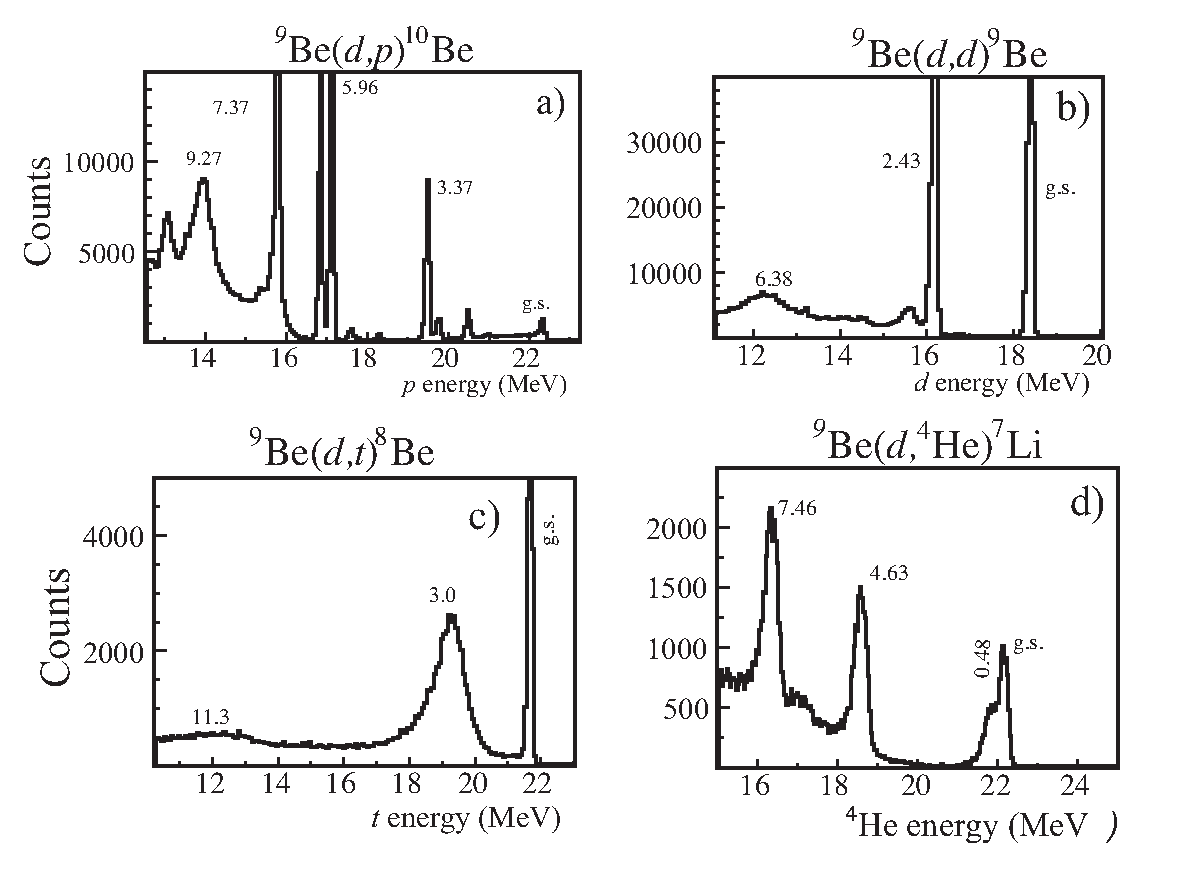
\includegraphics[width=8.2cm]{d_Etot_Fig2.eps}
\caption{Spectra of total deposited energy measured at $\theta_{lab}$=32$^\circ$ for the detected $p$ (panel a), $d$ (panel b), $t$ (panel c), and $\alpha$ (panel d). The ground and the excited states of ${}^7$Li for the detected complementary product $\alpha$ as well as the ground states and the excited states for ${}^8$Be, ${}^9$Be, and ${}^{10}$Be in the case of detected $t, d$, and $p$, as complementary products, respectively, are unambiguously identified.}
\label{fig2}
\end{figure}	

%%%%%%%%%%%%%%%%%%%%%%%%%%%%%%%%
The particles were identified based on the energy-loss measurements of $\Delta$E and the residual energy E$_r$, i.e., by the so-called $\Delta$E-E method. An example of two-dimensional plots (yield vs. energy loss $\Delta$E and residual energy E$_r$) is shown in Fig.~\ref{fig1}.

Current experimental technique allow identification of the particles $p, d, t$, and $\alpha$ and determination of their total deposited energies. The spectra of total deposited energies are shown in Fig.~2. All the peaks in Fig.~\ref{fig2} have been identified and assigned to the ground and excited states of ${}^{10}$Be, ${}^9$Be, ${}^8$Be, and ${}^7$Li nuclei as the complementary products for the detected particles $p, d, t$, $\alpha$, respectively.

\section{Data Analysis and Results }
\subsection{Elastic scattering}



% Please add the following required packages to your document preamble:
% \usepackage{booktabs}
\begin{table*}[bp]
\footnotesize
\caption{\label{potpar} Parameterized double-folding potentials of the $d$+$^9$Be system used in the OM, CC and DWBA calculations.}
\begin{tabular*}{\textwidth}{ll@{\extracolsep{\fill}}llllllllll}
\toprule
E$_d$, & i & V$_0$, & r$_v^{a}$, & a$_v$, & W$_0$, & r$_w^{a}$, & a$_w$, & V$_0^{SO}$, & N$_R$, & r$_C^{a}$, & $\chi^2$ \\
MeV   &   & MeV   & fm    & fm    & MeV   & fm    & fm    & MeV        &       & fm   						& \\ \midrule
19.5  & 1 & 6.18  & 0.328 & 0.308 & 3.99  & 0.328 & 0.127 & 3.275      & 1.22  & 0.809 			& 	2.490	\\
      & 2 & 70.97 & 0.746 & 0.831 & 25.50 (17.5$^{b}$) & 0.746 & 0.766 &            &       &    						&   \\
      & 3 & 0.605 & 1.491 & 1.724 & 0.924 & 1.491 & 2.238 &            &       &   							&    \\ \midrule
35.0  & 1 & 5.941 & 0.328 & 0.308 & 7.07  & 0.612 & 0.108 & 3.275      & 1.17  & 0.809 			&	2.503\\
      & 2 & 68.68 & 0.746 & 0.831 & 22.50 (17.5$^{b}$)& 0.838 & 0.731 &            &       &       						&\\
      & 3 & 0.58  & 1.491 & 1.724 & 0.999 & 1.377 & 1.856 &            &       &      							& \\ \bottomrule
\end{tabular*}
\scriptsize
$^{a}$ Radii are defined as $R_i = r_i \left( A^{1/3}_P+A^{1/3}_T \right)$.  \\
$^{b}$ The values are used in CRC calculations. \\
\end{table*}



The theoretical calculations  of the deuteron  elastic scattering  on  ${}^9$Be  at 19.5 and 35 MeV energies have been performed in the framework of the OM with the OM potential given by:

\begin{equation}\label{eqn:OP}
\begin{array}{l}
 U(R)=-V^{V}(R)-iW^{V}(R)+V^{SO}(R)( \mathbf{l} \cdot \sigma )\\
~~~ ~~~~~~~+V^C(R),
\end{array}
\end{equation}
where $V^{V}, W^{V}, V^{SO},$ and $V^C$ are real volume,  imaginary volume, spin-orbit and Coulomb potentials, respectively. In this work, the real part of the OM potential was obtained by means of the double-folding (DF) model
\begin{equation}
V^V(R) = N_R V^{DF}(R)
\end{equation}
with normalization factor $N_R$. For convenience, in the OM and CC (CRC) calculations the potential can be fitted by means of the sum of three Woods-Saxon potentials:
\begin{eqnarray}
V^V(R) =  \sum_{i=1}^{3} V^i f^{R_i, a_i}(R), \\
 f^{R_V,a_V}(R)=\frac{1}{1+exp{\frac{R-R_V}{a_V}}}.
\end{eqnarray}

\begin{figure}[tp]
\centering
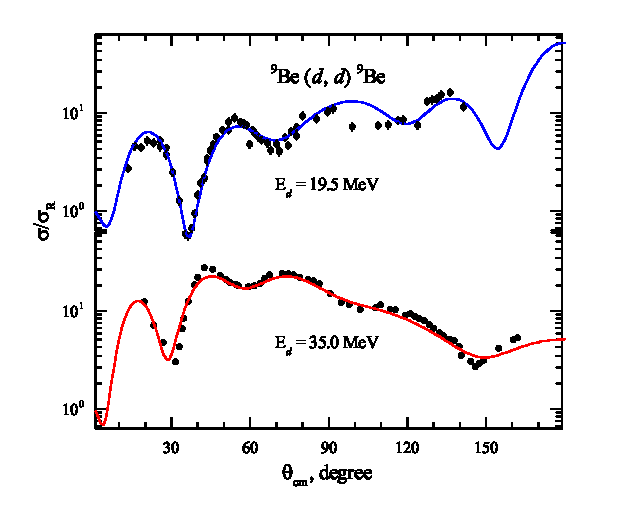
\includegraphics[width=8.2cm]{2H9BE_old.eps}
\caption{ \label{2H9BE_old} \footnotesize The angular distribution of elastic scattering data of $d$ from ${}^9$Be at laboratory energy 19.5~MeV in comparison with theoretical calculations within the OM (solid curve). }
\end{figure}

The DF potential was calculated using the effective M3Y-Paris nucleon-nucleon potential and the nuclear-matter-densities of projectile and target nuclei. In order to calculate the ${}^9$Be matter distribution we applied the $\alpha+\alpha+n$ three-body model (for more details, see Ref.~\cite{urazbekov2016}), while the matter density distribution of the deuteron projectile was chosen to be of the form
\begin{equation}
\rho\left( \frac{1}{2}r \right) =\int \vert \Psi (\textbf{r}) \vert d \Omega_r.
\end{equation}


%The surface and 
The spin-orbit term of the OM potential has standard form
\begin{eqnarray}
%W^D(R) &= -4 a_D W_0^D \frac{d}{dR} f^{R_D,a_D}(R), \\
V^{SO}(R) &= V_0^{SO}\left(\frac{\hbar}{m_\pi c}\right)^2 \frac{1}{R} \frac{d}{dR} f^{R_{SO} a_{SO}}(R).
\end{eqnarray}
The Coulomb term has been taken as the interaction of a point-charge with a uniformly charged sphere
\begin{eqnarray}
\label{coul}
V^C(R)=
\cases{
\frac{Z_1 Z_2 e^2}{2 R_C} \left( 3- \frac{R^2}{R_C^2} \right), & for  R $\leq R_C$, \\
\frac{Z_1 Z_2 e^2}{R}, & for  R $> R_C$ .
}
\end{eqnarray}

The parameters of the imaginary part of the optical potential were obtained by fitting the theoretical cross sections to the experimental data at 19.5 MeV and 35 MeV incident energies. As a starting point, the same parameterizations of the real part were used. The obtained potential parameters after fitting are listed in Table~\ref{potpar} for both 19.5 MeV and 35.0 MeV incident energies.

The comparison of the results of the theoretical calculations with  the measured data for elastic scattering at 19.5 MeV and 35.0 MeV energies are plotted in Fig.~\ref{2H9BE_old}. 
The cross sections obtained in the framework of the OM with the DF potential are shown as solid curves. 
Theoretical results obtained by means of the OM give an excellent agreement, $\chi^2\approx2.5$, with the experimental data. The  parameters of  parameterized double-folding potential are listed in Table \ref{potpar}. 

\begin{figure}[tp]
\centering
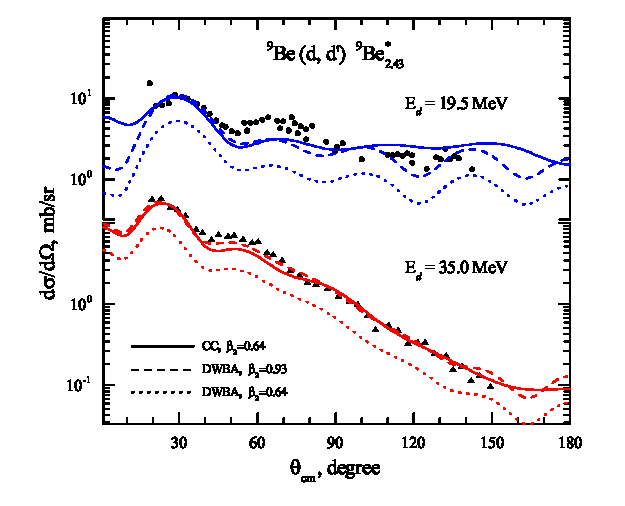
\includegraphics[width=8.2cm]{2H9BE2430MEV.eps}
\caption{\label{2H9BE2430MEV}The cross sections of inelastic scattering ${}^9$Be($d,d$)$^9$Be* (E$_{exc}$=2.43 MeV) at laboratory energies 19.5 MeV (full circle) and 35 MeV (full triangle). Theoretical curves are described in the text.}
\end{figure}

\subsection{Inelastic scattering}
The CC and DWBA approaches have been applied to analyse the measured inelastic scattering data corresponding to the ${}^9$Be($5/2^-, 2.43$ MeV) excitation. Calculations were performed employing the FRESCO code \cite{fresco} and the DWUCK5 code \cite{kunz} which are available in the NRV knowledge-base \cite{nrv}.

In order to describe the measured experimental data one has to consider the ${}^9$Be target having a quadrupole deformation. Thus, the ${}^9$Be spectrum consists of the rotational band including the  $3/2^-$ ground state, $5/2^-$ state at 2.43 MeV and $7/2^-$ state at 6.38 MeV. Couplings to these states were taken into account within the coupled-channel approach. The spin reorientations were also taken into account. The coupling interaction has the usual form:
\begin{equation}
V_\lambda(R)=-\beta_\lambda R_V \left|\frac{d V^V}{dR}\right| - i \beta_\lambda R_W \left|\frac{d W^D}{dR}\right|,
\end{equation}
where $\beta_\lambda$ is the deformation parameter of $\lambda$ multipole describing the target-nucleus form. Here, we neglect as usual the contribution of the Coulomb interaction.


The calculated cross sections for inelastic scattering to the $5/2^-$ state at 2.43 MeV are shown in Fig.~\ref{2H9BE2430MEV}. The solid curves correspond to the results obtained within the CC approach, while the dashed and dotted curves were obtained within the DWBA approach using  different values of the deformation parameter $\beta_2$. The used potential parameters are listed in Table~\ref{potpar}.

All the results in Fig.~\ref{2H9BE2430MEV} are in good agreement with the experimental data. The quadrupole deformation parameter $\beta_2 = 0.64$ extracted within the coupled-channel model is consistent with the previous studies \cite{lukyanov2014, harakeh1980}.

In the case of DWBA calculations, one uses the DF potential (see Table~\ref{potpar}) for both the entrance and the exit channels. The DWBA angular distributions very well reproduce the structure of experimental data but clearly underestimate them when the deformation parameter $\beta_2 = 0.64$ is used (see the dotted curves in Fig.~\ref{2H9BE2430MEV}). In order to get the best fit the deformation parameter must be increased up to $\beta_2 = 0.93$, which is quite close to the values reported in previous studies (see, for example, \cite{bodek1989, votava1973}).

\begin{figure}[bp]
\centering
\includegraphics[scale=0.85]{9BE8BECC.eps}
\caption{ \label{9BE8BECC} The target coupling schemes in the ${}^9$Be($d,p$)$^{10}$Be (upper) and the ${}^9$Be($d,t$)$^8$Be (lower) nuclear reactions. The bold two-headed arrows indicate E$\lambda$ transitions. The spin re-orientation effects are indicated as back-pointing arrows.}
\end{figure}	

Thus, one may confirm that channel coupling and the effects of spin reorientation enhance the cross section that results in the reduction of the deformation parameter. However, the DWBA approach takes into account only first-order contributions to the transition amplitude. In particular, it also describes only general features of the angular distributions and overestimates the deformation parameter in order to compensate the difference between the experimental data and the DWBA cross sections.

%The implementation of the CC approach is demonstrating a good agreement with angular distributions of inelastic scattering data. Exact matching value of the deformation parameter with other theoretical researches has been obtained. Generally it can be concluded that  strong coupling effects between channels exist in ${}^9$Be($d,d$)$^9$Be$^*$.
%In accordance with a good agreement of experimental data with both theoretical angular distributions and obtained deformation parameter within the CC approach it should therefore be noted that there exist strong coupling effects between channels.


\subsection{One-nucleon transfer reactions }
The one-neutron pick-up ${}^9$Be($d,t$)${}^8$Be and stripping ${}^9$Be($d,p$)${}^{10}$Be reactions were analyzed here within the framework of  the Coupled Reaction Channels (CRC).

\begin{figure}[tp]
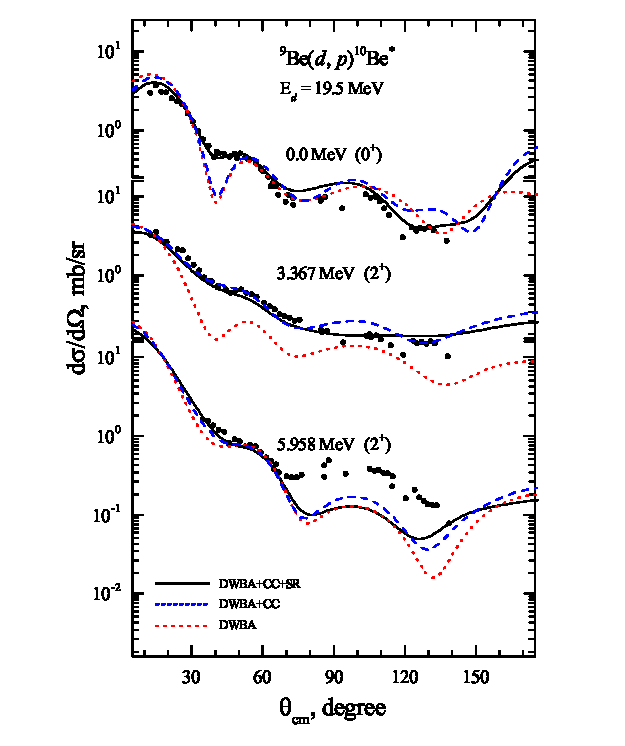
\includegraphics[scale=0.8]{1H10BE.eps}
\caption{\label{1H10BE} Differential cross sections for the ${}^9$Be($d,p$)${}^{10}$Be$^*$ reactions at 19.5 MeV leading to different final states (labelled in the figure) in ${}^{10}$Be. The experimental data are shown in comparison with theoretical results obtained within the CRC method.}
\end{figure}

\begin{figure}[tp]
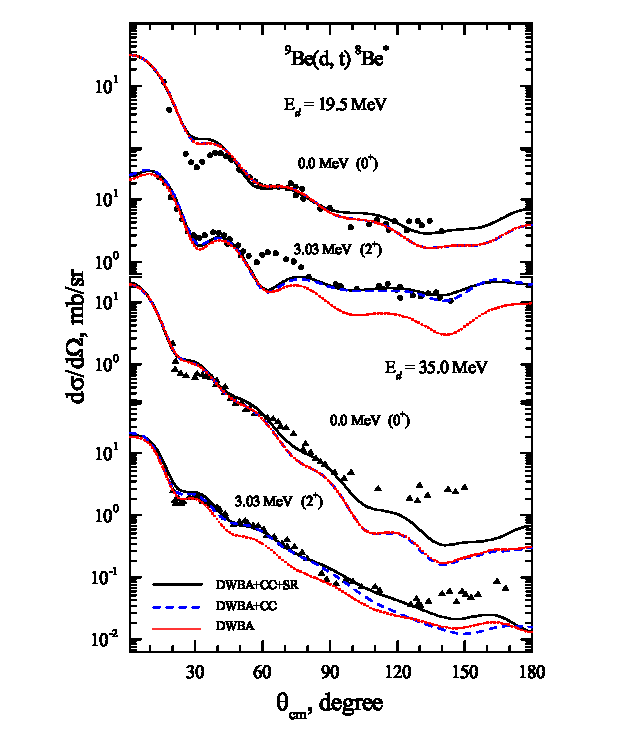
\includegraphics[scale=0.8]{3H8BE.eps}
\caption{
\label{3H8BE}
Differential cross sections for the ${}^9$Be($d,t$)${}^{8}$Be$^*$ reactions at 19.5 and 35 MeV leading to different final states (labelled in the figure) in ${}^{8}$Be. The experimental data are shown in comparison with  theoretical results obtained within the CRC method.}
\end{figure}

The double-folding potential given in Table \ref{potpar} was used in the CRC calculations for the entrance channel and the global optical parameterizations from Ref. \cite{globalProton, globalTriton} were used for the exit channels. The coupling schemes of target and daughter nuclei for the ${}^9$Be($d,p$)${}^{10}$Be and ${}^9$Be($d,t$)${}^8$Be  reactions  are illustrated in Fig. \ref{9BE8BECC}. The states of ${}^{10}$Be, $2^+_{1}$ and $2^+_{2}$, as well as the low-lying excited states of ${}^8$Be, $2^+$ and $4^+$, were included in the coupling scheme. Also, the schemes take into account the spin reorientations of states on the condition $J \neq 0$.

In order to construct the bound-state wave functions of the transferred particle in the entrance and exit channels, the common method, i.e. fitting the depth of the corresponding Woods-Saxon potential to the known binding energy, was employed. The reduced radius and diffuseness in this case are set to be $r = 1.25$ fm and $a$ = 0.65 fm, respectively. If the transfer takes place to a final unbound state, the depth of the potential for this state was adjusted to yield a binding energy equal to $-0.1$ MeV in accordance with the procedure used in Ref. \cite{harakeh1980}.

%If the core and the composite nuclei have internal excitation energies, a renewed binding energy $BE^{\star}$ of the transferred particle is expressed by the formula:
%\begin{equation} BE^{\star}=BE - E_{com}^*+E_{core}^* \end{equation}
%where $BE$ $-$ the binding energy of the transferred particle, $E_{com}^*,~E_{core}^*~-$  excitation energies of the composite and  core nuclei, respectively.

The spectroscopic amplitude  $\mathcal{S}$ for the addition of a particle to a core with angular momentum $J_{core}$ to form a composite with $J_{com}$ is related to the matrix element of the creation operator~$\hat{a}^\dagger$:
%\cite{brown2017}:
\begin{eqnarray}\label{eq:SA}
\mathcal{S}_{Nlj} = \frac{\langle J_{com} \| \hat{a}^\dagger _{Nlj} \| J_{core}  \rangle}{\sqrt{2J_{com}+1}}
%= (-)^{j+J-J'} \frac{\langle J_{core}  \| \hat{a} _{NL_J} \| J_{com}  \rangle}{\sqrt{2J+1}}
\end{eqnarray}
where $Nlj$ is the set of particle quantum numbers. The spectroscopic amplitudes for one particle states were calculated by means of the $ANTOINE$ code \cite{antoine}  using the effective Cohen-Kurath interaction for $p$-shell nuclei \cite{cohen1965}. The calculated spectroscopic amplitudes for the one-nucleon transfer reactions are listed in Table~\ref{SA}.

\begin{table*}[tp]
\footnotesize
\caption{\label{SA} Spectroscopic amplitudes used in CRC calculations for the Composite = Core + Cluster system. The one-nucleon spectroscopic amplitudes have been calculated by means of the $ANTOINE$ code \cite{antoine}. The alpha spectroscopic amplitudes were taken from  \cite{volya, volya2017}. }
\begin{tabular*}{\textwidth}{@{\extracolsep{\fill}}llllllrl@{\extracolsep{\fill}}llllllr@{\extracolsep{\fill}}}
\br
Composite & 2J$_{com}$ & Core & 2J$_{core}$ & Cluster & 2J & SA &    & Composite & 2J$_{com}$ & Core & 2J$_{core}$ & Cluster & 2J & SA      \\
\mr
$^9$Be  & 3  & ${}^8$Be   & 0   & $n$       & 3   & $-$0.761 &  & ${}^9$Be  & 3  & ${}^8$Li   & 2$_1$    & $p$       & 1   & $-$0.444  \\
$^9$Be  & 3  & ${}^8$Be   & 4   & $n$       & 3   & 0.816  &  & ${}^9$Be  & 3  & ${}^8$Li    & 6   & $p$       & 3   & $-$0.592  \\
$^9$Be  & 3  & ${}^8$Be   & 4   & $n$       & 1   & $-$0.242 &  & ${}^9$Be  & 3  & ${}^8$Li    & 2$_2$   & $p$       & 3   & $-$0.236  \\
$^9$Be  & 5  & ${}^8$Be   & 4   & $n$       & 3   & 0.986  &  & ${}^9$Be  & 3  & ${}^8$Li    & 2$_2$   & $p$       & 1   & 0.036   \\
$^9$Be  & 5  & ${}^8$Be   & 4   & $n$       & 1   & $-$0.417 &  & ${}^9$Be  & 5  & ${}^8$Li    & 4   & $p$       & 3   & 0.593   \\
$^9$Be  & 5  & ${}^8$Be   & 8   & $n$       & 3   & $-$0.374 &  & ${}^9$Be  & 5  & ${}^8$Li    & 4   & $p$       & 1   & 0.515   \\
$^9$Be  & 7  & ${}^8$Be   & 4   & $n$       & 3   & $-$0.457 &  & ${}^9$Be  & 5  & ${}^8$Li   & 2$_1$    & $p$       & 3   & $-$0.672  \\
$^9$Be  & 7  & ${}^8$Be   & 8   & $n$       & 3   & 0.919  &  & ${}^9$Be  & 5  & ${}^8$Li    & 6   & $p$       & 3   & $-$0.571  \\
$^9$Be  & 7  & ${}^8$Be   & 8   & $n$       & 1   & $-$0.429 &  & ${}^9$Be  & 5  & ${}^8$Li    & 6   & $p$       & 1   & $-$0.171  \\
$^8$Be  & 0  & ${}^7$Li   & 3   & $p$       & 3   & $-$1.204 &  & ${}^9$Be  & 5  & ${}^8$Li    & 2$_2$   & $p$       & 3   & 0.200     \\
$^8$Be  & 0  & ${}^7$Li   & 1   & $p$       & 1   & 0.736  &  & ${}^9$Be  & 7  & ${}^8$Li    & 4   & $p$       & 3   & $-$0.323  \\
$^8$Be  & 4  & ${}^7$Li   & 3   & $p$       & 3   & $-$0.748 &  & ${}^9$Be  & 7  & ${}^8$Li    & 6   & $p$       & 3   & $-$0.899  \\
$^8$Be  & 4  & ${}^7$Li   & 3   & $p$       & 1   & $-$0.612 &  & ${}^9$Be  & 7  & ${}^8$Li    & 6   & $p$       & 1   & $-$0.564  \\
$^8$Be  & 4  & ${}^7$Li   & 1   & $p$       & 3   & 0.667  &  & ${}^7$Li  & 3  & ${}^6$Li   & 2   & $n$       & 3   & 0.657   \\
$^8$Be  & 4  & ${}^7$Li   & 7   & $p$       & 3   & 0.624  &  & ${}^7$Li  & 3  & ${}^6$Li   & 2   & $n$       & 1   & $-$0.538  \\
$^8$Be  & 4  & ${}^7$Li   & 5$_2$   & $p$       & 3   & 0.079  &  & ${}^7$Li  & 3  & ${}^6$Li   & 6   & $n$       & 3   & 0.744   \\
$^8$Be  & 4  & ${}^7$Li   & 5$_2$   & $p$       & 3   & $-$0.146 &  & ${}^7$Li  & 3  & ${}^6$Li   & 4   & $n$       & 3   & $-$0.032  \\
$^8$Be  & 8  & ${}^7$Li   & 7   & $p$       & 3   & 0.864  &  & ${}^7$Li  & 3  & ${}^6$Li   & 4   & $n$       & 1   & 0.399   \\
$^8$Be  & 8  & ${}^7$Li   & 7   & $p$       & 1   & 0.687  &  & ${}^7$Li  & 1  & ${}^6$Li   & 2   & $n$       & 3   & $-$0.925  \\
$^8$Be  & 8  & ${}^7$Li   & 5$_2$   & $p$       & 3   & 0.374  &  & ${}^7$Li  & 1  & ${}^6$Li   & 2   & $n$       & 1   & 0.197   \\
$^8$Li  & 4  & ${}^7$Li   & 3   & $n$       & 3   & $-$0.988 &  & ${}^7$Li  & 1  & ${}^6$Li   & 4   & $n$       & 3   & $-$0.555  \\
$^8$Li  & 4  & ${}^7$Li   & 3   & $n$       & 1   & 0.237  &  & ${}^7$Li  & 7  & ${}^6$Li   & 6   & $n$       & 3   & $-$0.936  \\
$^8$Li  & 4  & ${}^7$Li   & 1   & $n$       & 3   & 0.430   &  & ${}^7$Li  & 7  & ${}^6$Li   & 6   & $n$       & 1   & 0.645   \\
$^8$Li  & 4  & ${}^7$Li   & 7   & $n$       & 3   & $-$0.496 &  & ${}^7$Li  & 7  & ${}^6$Li   & 4   & $n$       & 3   & $-$0.456  \\
$^8$Li  & 4  & ${}^7$Li   & 5   & $n$       & 3   & $-$0.665 &  & ${}^7$Li  & 5$_2$  & ${}^6$Li   & 2   & $n$       & 3   & $-$0.650   \\
$^8$Li  & 4  & ${}^7$Li   & 5$_2$   & $n$       & 1   & $-$0.275 &  & ${}^7$Li  & 5$_2$  & ${}^6$Li   & 6   & $n$       & 3   & 0.732   \\
$^8$Li  & 2$_1$  & ${}^7$Li   & 3   & $n$       & 3   & 0.567  &  & ${}^7$Li  & 5$_2$  & ${}^6$Li   & 6   & $n$       & 1   & 0.549   \\
$^8$Li  & 2$_1$  & ${}^7$Li   & 3   & $n$       & 1   & 0.351  &  & ${}^7$Li  & 5$_2$  & ${}^6$Li   & 4   & $n$       & 3   & 0.200     \\
$^8$Li  & 2$_1$  & ${}^7$Li   & 1   & $n$       & 3   & 0.905  &  & ${}^7$Li  & 5$_2$  & ${}^6$Li   & 4   & $n$       & 1   & $-$0.114  \\
$^8$Li  & 2$_1$  & ${}^7$Li   & 1   & $n$       & 1   & 0.331  &  & ${}^6$Li  & 2  & $d$     & 2   & $\alpha$     & 0   & 0.907  \\
$^8$Li  & 2$_1$  & ${}^7$Li   & 5$_2$   & $n$       & 3   & 0.767  &  & ${}^6$Li  & 2  & $d$     & 2   & $\alpha$     & 4   & 0.077   \\
$^8$Li  & 6  & ${}^7$Li   & 3   & $n$       & 3   & 0.581  &  & ${}^6$Li  & 6  & $d$     & 2   & $\alpha$     & 4   & 0.943   \\
$^8$Li  & 6  & ${}^7$Li   & 5$_2$   & $n$       & 3   & $-$0.660  &  & ${}^6$Li  & 6  & $d$     & 2   & $\alpha$     & 8   & 0.028   \\
$^8$Li  & 6  & ${}^7$Li   & 5$_2$   & $n$       & 1   & $-$0.541 &  & ${}^6$Li  & 4  & $d$     & 2   & $\alpha$     & 4   & 0.929   \\
$^8$Li  & 6  & ${}^7$Li   & 7   & $n$       & 3   & 0.973  &  & ${}^9$Be  & 3  & ${}^5$He   & 3   & $\alpha$     & 0   & $-$0.925  \\
$^8$Li  & 6  & ${}^7$Li   & 7   & $n$       & 1   & $-$0.404 &  & ${}^9$Be  & 3  & ${}^5$He   & 3   & $\alpha$     & 4   & 0.784   \\
$^8$Li  & 2$_2$  & ${}^7$Li   & 3   & $n$       & 3   & $-$0.617 &  & ${}^9$Be  & 5  & ${}^5$He   & 3   & $\alpha$     & 4   & 0.974   \\
$^8$Li  & 2$_2$  & ${}^7$Li   & 3   & $n$       & 1   & $-$0.841 &  & ${}^9$Be  & 5  & ${}^5$He   & 3   & $\alpha$     & 8   & $-$0.260   \\
$^8$Li  & 2$_2$  & ${}^7$Li   & 1   & $n$       & 3   & 0.178  &  & ${}^9$Be  & 7  & ${}^5$He   & 3   & $\alpha$     & 4   & 0.882   \\
$^8$Li  & 2$_2$  & ${}^7$Li   & 1   & $n$       & 1   & 0.331  &  & ${}^9$Be  & 7  & ${}^5$He   & 3   & $\alpha$     & 8   & $-$0.737  \\
$^8$Li  & 2$_2$  & ${}^7$Li   & 5   & $n$       & 3   & 0.231  &  & ${}^7$Li  & 3  & $t$     & 1   & $\alpha$     & 1   & 0.970       \\
$^9$Be  & 3  & ${}^8$Li    & 4   & $p$       & 3   & $-$0.947 &  & ${}^7$Li  & 1  & $t$     & 1   & $\alpha$     & 1   & 0.961       \\
$^9$Be  & 3  & ${}^8$Li    & 4   & $p$       & 1   & $-$0.319 &  & ${}^7$Li  & 7  & $t$     & 1   & $\alpha$     & 3   & 0.952       \\
$^9$Be  & 3  & ${}^8$Li    & 2$_1$   & $p$       & 3   & 0.454  &  & ${}^7$Li  & 5$_2$  & $t$     & 1   & $\alpha$     & 3   & 0.223  \\
\br
\end{tabular*}
\end{table*}

\begin{figure*}[bp]
\centering
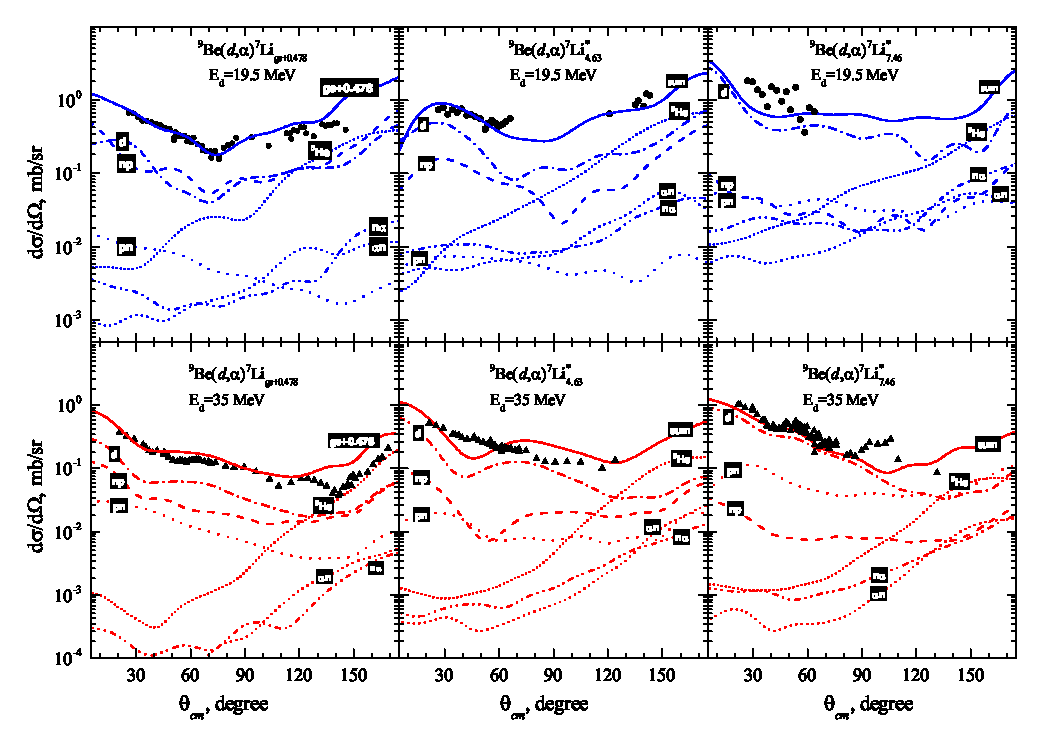
\includegraphics[scale=0.9]{4HE7LI.eps}
\caption{\label{label} Differential cross sections for the ${}^9$Be($d$,$\alpha$)${}^7$Li reactions measured at 19.5 MeV and 35 MeV energy with the ${}^{7}$Li observed in the ground or low-lying excited states in the exit channels.}
\label{4HE7LI}
\end{figure*}	

Angular distributions of the ${}^9$Be($d,p$)${}^{10}$Be nuclear reaction at E$_d$=19.5 MeV are shown in comparison with the theoretical curves  calculated in the framework of the CRC method in Fig. \ref{1H10BE}.

In order to study the couplings of the input  channels, the outputs  were fixed using the deformation parameter of $^8$Be from Ref. \cite{rocca2018}, and for $^{10}$Be from Ref. \cite{harakeh1980}. 
The direct transition from the ground state is indicated by the dotted line (DWBA). 
The contributions of the transitions from excited states (CC), and from spin reorientations (SR) are indicated by dashed and solid lines, respectively.
During the analysis, it was found that spin reorientation has a significant contribution in the $p$ + $^{10}$Be$_{gs}$ channel, especially in the range of 40-60 degrees. 
It is interesting to note that we managed to describe within the CRC method the differential cross section of the ${}^9$Be($d,p$)${}^{10}$Be$_{gs}$ reaction at all scattering angles, including the range 40$^\circ$-60$^\circ$, where they were not covered in Refs. \cite{galanina2012, bodek1989}.
 
An appreciable contribution of the \begin{small}
$3/2^- \rightarrow 2^+_1,~5/2^- \rightarrow 2^+_1,~7/2^-\rightarrow 2^+_1$
\end{small} transitions was observed in the $p$~+~$^{10}$Be$_{3.37}$ channel in the entire range of scattering angles. 
In the cross section of the  $p$~+~$^{10}$Be$_{5.96}$ channel, the theoretical calculation underestimates the experimental data starting from 70$^\circ$. Possibly, other higher excited states of $^9$Be should be taken into account.

Figure \ref{3H8BE} displays the cross sections of the ${}^9$Be($d,t$)${}^{8}$Be nuclear reaction at both 19.5 MeV and 35 MeV incident energies. As in the case of the ($d,p$) reactions, the ($d,t$) reactions also show the strong channel-coupling effects. We see a manifestation of spin-reorientation effects in the $t$+$^8$Be$_{gs}$ channels and a significant contribution of the  \begin{small}
$3/2^- \rightarrow 2^+,~ 5/2^- \rightarrow 2^+,~ 7/2^-\rightarrow 2^+$
\end{small} transitions in the $t$+$^8$Be$_{3.03}$ channel.

Theoretical calculations made within the CRC method show good agreement with the experimental data for both ($d,p$)  and ($d,t$) reactions.
The analysis showed strong coupling effects in both entrance and exit channels. The effects of such couplings were also emphasized in Refs. \cite{harakeh1980, rudchik2016}.

\begin{figure}[tp]
\centering
\includegraphics[scale=0.8]{4HE7LiCC.eps}
\caption{\label{4He7LICC} The scheme illustrates the reaction mechanisms taken into account in CRC calculations of the cross sections for ${}^9$Be($d,\alpha$)${}^7$Li reaction.}
\end{figure}

\subsection{Cluster-transfer reaction}
Differential cross sections for the nuclear reaction ${^9}$Be($d,\alpha$)${}^7$Li are of particular interest. This is due to the specific behaviour of the cross section at large scattering angles, which indicates a ${}^5$He cluster transfer. In addition, the cross section calculated within the DWBA approach underestimates the data even at forward scattering angles. Therefore, in order to understand the difference between theory and experiment, the following transfer mechanisms are suggested (see Fig. \ref{4He7LICC}):
\begin{itemize}
\item[$-$] direct transfer of heavy clusters $d$ and ${}^5$He;
\item[$-$] sequential two-step transfer of $n$-$p$, $p$-$n$, $n$-$\alpha$ and $\alpha$-$n$;
\end{itemize}

The resulting differential cross section for the ${^9}$Be($d$,$\alpha$)${}^7$Li reaction has the form of a coherent sum of two amplitudes
\begin{equation}
\frac{d\sigma}{d\Omega}(\theta) =\vert f_{I}(\theta) + f_{II}(\theta) \vert ^2,
\end{equation}
where the amplitude
\begin{equation} \label{eq:ampl1}
f_{I}(\theta)=f_{{}^5\textrm{He}}(\pi - \theta) + f_{n\textrm{-}\alpha}(\pi - \theta) + f_{\alpha\textrm{-}n}(\pi - \theta)
\end{equation}
describes the transfer of the heavy ${}^5$He-cluster and sequential two-step transfer of n-$\alpha$ and $\alpha$-n, and the amplitude
\begin{equation} \label{eq:ampl2}
f_{II}(\theta)=f_{d}(\theta) + f_{n\textrm{-}p}( \theta) + f_{p\textrm{-}n}(\theta)
\end{equation}
corresponds to the deuteron pick-up and sequential two-step transfer of $n$-$p$ and $p$-$n$.

The DF potential (see Table~\ref{potpar}) for the entrance channel and global optical potential parameterizations from Refs. \cite{globalTriton, globalAlpha, global6Li} for intermediate and exit channels were used in the analysis.
The prior form for the first coupling and the post form for the second coupling were chosen for two-step transfer reactions in order to avoid the non-orthogonal terms in the calculations of transition amplitudes.

%Important ingredients of the CRC method are the spectroscopic amplitudes of the composite configurations in the entrance, exit and intermediate states. In order to calculate the one nucleon spectroscopic amplitudes we applied the \textit{ANTOINE} code \cite{antoine} that reproduces the excitation functions of all p-shell nuclei well.

The spectroscopic amplitudes of the $d$ and ${}^5$He clusters were taken from Ref. \cite{fiveSA}, while the alpha-cluster spectroscopic amplitudes given in Table~\ref{SA} were provided by Dr. A. Volya within the method reported in Ref. \cite{volya2017}.

The calculated cross sections are shown in Fig.~\ref{4HE7LI} with the $\alpha$-particle angular distributions formed in the ${}^9$Be(d,$\alpha$)${}^7$Li$^*$ reaction at incident energies of 19.5 and 35 MeV and corresponding to the low-lying excitation of the ${}^7$Li nucleus in the exit channels. The transfer of the deuteron (dash-dotted curve) provides the dominant contribution in all the channels. Despite the fact that the spectroscopic amplitude of the deuteron $\mathcal{S}_{1{D}_3}=0.558$ in the ${}^9$Be nucleus is not of great importance, a noticeable cross section is due to the large value of the deuteron spectroscopic amplitude $\mathcal{S}_{1{S}_1}=1.732$  of ${}^4$He.

The angular distribution of deuteron transfer has a significant cross section also at the backward scattering angles, which is mainly caused by the contribution of the $D$ wave. This symmetrical behaviour of the cross section of $D$ waves is very similar to the cross section of evaporation residues. Tanaka \etal \cite{tanaka1978} analyzed the role of the compound process in ${}^9$Be($d,\alpha$)${}^7$Li reaction and claimed the domination of the compound nucleus channels at the energies of 12.17 MeV and 14.43 MeV. However, in Ref. \cite{bodek1989} the negligible contribution of the compound-nucleus mechanism was shown at 7 MeV using the DWBA analysis. In this regard, our theoretical results based on the CRC method show that there is no need to take into account the mechanism through the compound-nucleus formation at energies of 19.5 and 35.0 MeV.

Starting from scattering angle $\theta_{c.m.} =$ 120$^\circ$, the transfer of the ${}^5$He cluster, labeled as ${}^5$He in Fig. \ref{4HE7LI}, has a predominant contribution in all channels. It should be noted that a similar result was reported earlier in Ref. \cite{bodek1989}. One-step transfer of the ${}^5$He cluster was also indicated as a dominant process by Jarczyk \etal \cite{jarczyk1996} in studying the ${}^{12}$C(${}^{11}$B,${}^6$Li)${}^{17}$O and ${}^{12}$C($d$,${}^7$Li)${}^{7}$Be reactions.

Using the CRC method, we are able to estimate the contribution of the sequential transfer of ${}^5$He, which was not studied before. Corresponding cross sections are shown in Fig.~\ref{4HE7LI} as curves labeled $n\alpha$ and $\alpha n$.
It turned out that the $n$-$\alpha$ and $\alpha$-$n$ transfer processes provide indeed a contribution more than one order of magnitude smaller in comparison with the one-step ${}^5$He transfer. Nevertheless, it should be noted that the contribution of the $n$-$\alpha$ and the $\alpha$-$n$ transfer channels increases with the increase in the ${}^7$Li excitation energy, where they should not be ignored.

\begin{figure}%[tp]
\centering
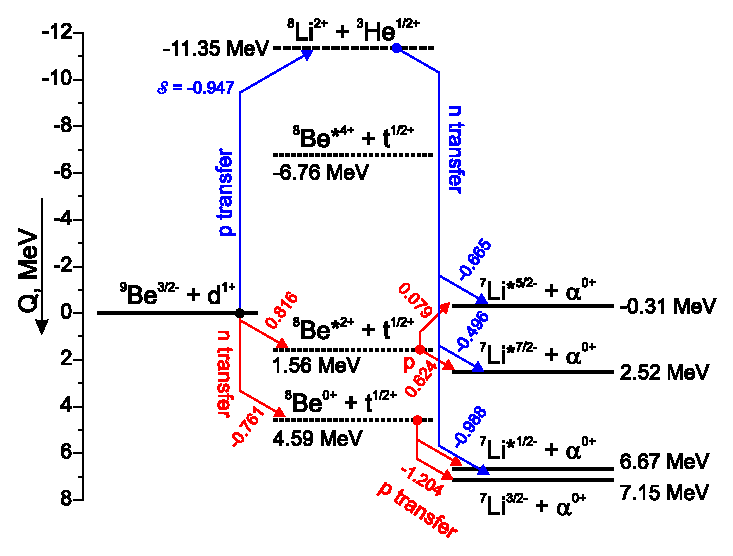
\includegraphics[width=230pt]{pnvsnp.eps}
\caption{\label{fig:pnvsnp} The scheme illustrates the energy balance of the different intermediate stages for the two-step mechanisms of ${}^9$Be($d,\alpha$)${}^7$Li transfer reaction. The $Q$-values for the different intermediate channels are shown near the corresponding lines. The numbers near the arrows correspond to the spectroscopic amplitudes of the heaviest reaction participants. For example, spectroscopic amplitude for the ${}^9$Be = ${}^8$Li + $p$ configuration is equal $\mathcal{S} = -0.947$.}
\end{figure}

The two-step $n$-$p$ transfer is another mechanism providing a noticeable contribution to the cross section. It is due to the prominent cluster structure of the ${}^9$Be nucleus having the weakly bound neutron. This structural feature explains also the weakness of the $p$-$n$ sequential transfer contribution to the cross section corresponding to the ${}^7$Li(g.s.) in the exit channel. However, with increasing the ${}^7$Li excitation energy these two mechanisms are interchanged in the significance of their contributions, as depicted by the curves in Fig.~\ref{fig:pnvsnp}, and the $p$-$n$ transfer begins to play a leading role, providing, in particular, almost 10 times larger contribution in the case of reaction at $E_{lab}$ = 35 MeV with ${}^7$Li$^*$(7.46 MeV) in exit channel.

In Fig.~\ref{fig:pnvsnp}, the possible scenarios for the $n$-$p$ and $p$-$n$ sequential transfer for the reaction under consideration are shown in respect to the $Q$-values. One may see that all the steps of the $n$-$p$ sequential transfer have positive $Q$-values, while the $p$-$n$ transfer goes through the intermediate channel ${}^8$Li + ${}^3$He that has a considerably negative $Q$-value. Together with the large values of the spectroscopic amplitudes (shown near to the arrows in Fig. \ref{fig:pnvsnp}), this explains the leading role of the ($d,t;t,\alpha$) mechanism in populating the ground state of ${}^7$Li in the exit channel.

\begin{figure}[tp]
\centering
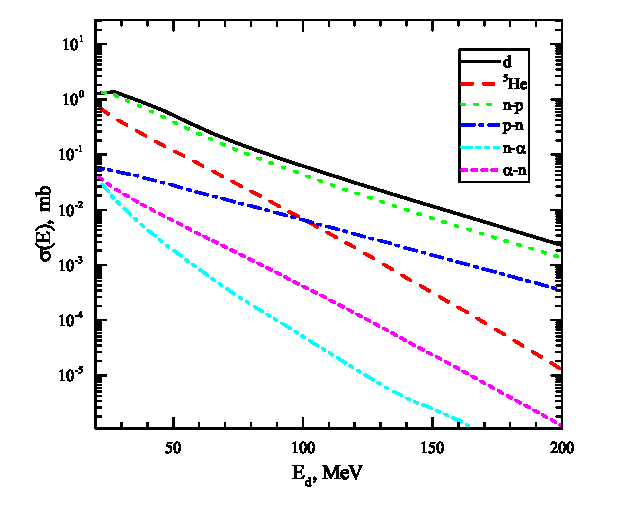
\includegraphics[width=8.2cm]{CS.eps}
\caption{\label{CS} Contributions of the different mechanisms to the cross section of the ${}^9$Be($d,\alpha$)${}^7$Li$_{g.s.}$ reaction. See Fig.~\ref{4He7LICC} for explanation of the curve notations.}
\end{figure}	

The situation becomes quite different in the case of the ${}^7$Li$^*$(5/2$^-$) in the exit channel. First, the population of this state through the $n$-$p$ transfer involves the ${}^9$Be~=~${}^8$Be$^*(2^+)$~+~$n$ intermediate configuration where the ${}^8$Be cluster has to be in the $2^+$ excited state. Note that the ${}^8$Be($0^+$) ground state is inappropriate because of angular-momentum-coupling mismatch in the entrance and exit configurations. Second, the extremely small spectroscopic amplitude of the ${}^8$Be$^*(2^+)$~=~${}^7$Li$^*(5/2^-)$~+~$p$ configuration, which is $\mathcal{S} = 0.079$, influences the transfer amplitude. These two factors lead to the suppression of the contribution of ($d,t;t,\alpha$) mechanism in population of the ${}^7$Li$^*$(5/2$^-$) state in the exit channel. Therefore, the $p$-$n$ sequential transfer prevails over the $n$-$p$ one. 

Figure \ref{CS} shows the contributions of all the mechanisms mentioned above to the total cross section of the ${}^9$Be($d,\alpha$)${}^7$Li$_{g.s.}$ reaction (see Fig.~\ref{4He7LICC}) as a function of the deuteron energy. One may conclude that mainly four mechanisms contribute to the cross section of this reaction. The transfer of the deuteron-cluster is the predominant channel at all collision energies. The sequential $n$-$p$ and $p$-$n$ transfers play a significant role at the high energies. The ${}^5$He-cluster transfer gives almost 20\% of the cross section at low energies and outdoes the sequential $p$-$n$ transfer in this energy domain. This allows us to claim that the configurations $n+^8$Be and $\alpha+{}^5$He provide noticeable contributions to the ground-state wave function of the ${}^9$Be nucleus. These conclusions agree well with the previous experimental studies \cite{brown2007, papka2007}.


	
\section{Conclusion}
In the present work, the deuteron-induced reactions on a ${}^9$Be target have been studied at the collision energies 19.5 and 35 MeV.  
The calculated double-folding potential has been applied successfully in describing the cross sections of elastic and inelastic scatterings, one-nucleon  transfer and cluster-transfer reactions.
  The deformation parameter for the transition \begin{small}
  $3/2^-\rightarrow5/2^-$
\end{small}  of ${}^9$Be has been determined.
 The strong coupling effects have been shown for the ($d,p$) and ($d,t$) one-nucleon transfer nuclear reactions.
 Furthermore, it was found that  in the ${}^9$Be($d$,$\alpha$)${}^7$Li nuclear reaction the ${}^5$He heavy cluster  is transferred mainly simultaneously, and the contribution of its sequential transfer is an order of magnitude lower.
 The importance of taking into account the mechanism of sequential transfer of the $n$-$p$ system has been revealed.
 Based on these observations from studying the interaction of the  deuteron with  $^9$Be, it can be concluded that the $^9$Be  nucleus has cluster structure.


\ack
	The authors acknowledge the support of the CANAM project \cite{canam} for providing beam time for the experiment. The authors are also grateful to I. Thompson for advising on the FRESCO code and to A. Volya for providing the alpha spectroscopic amplitudes.

This work was supported by the Russian Science Foundation (17-12-01170).



\section*{References}
\bibliographystyle{iopart-num}

\bibliography{urazbekov}
\end{document} 
